\documentclass[../thesis.tex]{subfiles}

\begin{document}

\chapter{Алгоритм обнаружения} \label{chapter:algorithm}

В этой главе подробно описывается разработанный алгоритм обнаружения скомпрометированых коммутаторов в ПКС.

\section{Общее описание предложенного алгоритма}

Алгоритм обнаружения скомпрометированных коммутаторов основан на анализе сетевой статистики, предоставляемой счетчиками, установленными на правилах маршрутизации.

Идея алгоритма заключается в том, что, используя информацию об установленных правилах маршрутизации в сети, имеющуюся на контроллере, возможно проверить корректность сетевой статистики, получаемой от коммутаторов.
А именно, проверить корректность значений счетчиков правил маршрутизации.

Некорректные значения счетчиков правил маршрутизации, передаваемых коммутатором контроллеру, могут быть получены в следствие атак на \textit{data-plane}, проводимых при помощи скомпрометированных коммутаторов.
Из классификации атак на \textit{data-plane}, приведенной в главе \ref{chapter:problem}, следует, что атаки производятся при помощи добавления новых или удаления существующих правил маршрутизации.
При этом контроллер не получает информацию о таких изменениях, если злоумышленник пытается скрыть факт наличия атаки.

Таким образом, представление контроллера о состоянии сети отличается от её реального состояния.
А значит и модельные графы зависимостей правил, описывающие реальную сеть и представление сети, имеющееся на контроллере, будут отличаться.

Такие атаки, как сброс пакетов, дублирование трафика или некорректная маршрутизация, изменяют множества доменных путей модельного графа, так как они создают/удаляют маршруты в сети.

Если множества доменных путей различаются, то по теореме \ref{th:flow_decomposition} следует, что значения потоковых функций на вершинах двух модельных графов будут отличны.
Такие потоковые функции на вершинах графа описывают значение счетчиков правил маршрутизации, установленных в сети.
Следовательно, атаки, проводимые при помощи скомпрометированных коммутаторов, будут приводить к некорректным значениям счетчиков правил маршрутизации.
Под некорректностью понимается наличие значений, которые не совпадают со значениями потоковых функций в графе, описывающем представление контроллера о сети.

Таким образом, необходим алгоритм проверки корректности счетчиков правил маршрутизации.
Такой алгоритм может быть реализован с использованием алгоритма предсказания значений потока через вершину графа зависимостей правил (алгоритм \ref{alg:flow_propagation}).
Алгоритм проверки выглядит следующим образом: 
\begin{itemize}
\item Предсказываются значения счетчиков правил маршрутишации.
\item Предсказанные значения сравниваются с реальными.
\end{itemize}

Если значения счетчиков отличаются больше чем на заданный допустимый порог, то фиксируется наличие атаки.
Алгоритм также учитывает легитимные потери пакетов, связанные с перегрузками в сети.

Использование алгоритма предсказания значений счетчиков предполагает наличие путевой развертки, описывающей доменные пути.
Путевая развертка строится при помощи алгоритма \ref{alg:create_path_scan} на основе графа зависимостей правил, который в свою очередь может быть построен при помощи анализа OpenFlow сообщений, проходящих между контроллером и коммутаторами.

Для предсказания значений счетчиков правил маршрутизации также необходимо необходимо проанализировать сетевую статистику -- то есть\linebreak узнать значения потоковой функции на доменных путях.
Для этого нужно установить в сеть дополнительные правила маршрутизации, поля \textit{match} которых определяются доменными путями.
Эти правила предназначены для подсчета количества пакетов с заголовками, определенными доменными путями.

Таким образом алгоритм состоит из двух основных фаз:
\begin{enumerate}
\item Установка дополнительных правил;
    \begin{itemize}
    \item Построение графа зависимостей правил;
    \item Построение путевой развертки;
    \item Создание дополнительных правил;
    \item Установка приоритетов;
    \item Установка правил.
    \end{itemize}
\item Анализ сетевой статистики.
    \begin{itemize}
    \item Предсказание значений счетчиков;
    \item Обнаружение скомпрометированных коммутаторов.
    \end{itemize}
\end{enumerate}

\pagebreak

\section{Установка дополнительных правил}

Первая фаза алгоритма обнаружения скомпрометированных коммутаторов предполагает установку в сеть дополнительных правил маршрутизации.

Каждое такое правило маршрутизации ставится в соответствие некоторому доменному пути из путевой развертки, который определяет поля \textit{match} этих правил маршрутизации.
Поля \textit{match} устанавливаются таким образом, чтобы дополнительные правила обрабытывали только пакеты из соответствующих им доменных путей.
Это необходимо для того, чтобы счетчики дополнительных правил маршрутизации отражали значения потоковых функций на доменных путях.

Для того, чтобы определить вид дополнительных правил, необходимо построить путевую развертку, которая описывает доменные пути.
Путевая развертка сроится по алгоритму \ref{alg:create_path_scan} на основе графа зависимостей правил, описывающего доменные пути.

\subsection{Построение графа зависимостей правил}

Граф зависимостей правил строится инкрементально на основе событий изменения состояния сети. События изменения сети описываются OpenFlow сообщениями, передаваемыми между контроллером и коммутаторами. Такие события включают:
\begin{enumerate}
\item Подключение нового коммутатора;
\item Отключение существующего коммутатора;
\item Обнаружение физической линии между коммутаторами;
\item Обрыв физической линии между коммутаторами;
\item Установку нового правила маршрутизации;
\item Удаление существуюшего правила маршрутизации.
\end{enumerate}

Каждое описанное выше событие добавляет или удаляет некоторый набор вершин графа зависимостей правил.
При добавлении/удалении вершины также изменяется набор ребер графа.
Опишем более подробно процесс изменения ребер графа.

\subsubsection{Подключение/отключение коммутатора}

При появлении нового коммутатора создается следующий набор вершин:
\begin{itemize}
\item Стоковые вершины;
\item Истоковые вершины;
\item Вершины, соответствующие правилам по-умолчанию.
\end{itemize}

Пара стоковых и истоковых вершин создается для каждого порта коммутатора.
Этими правилами описываются получатели и генераторы трафика.
Также добавляются вершины, соответствующие правилам по-умолчанию для каждой таблицы коммутатора.
Такие правила описывают действия над пакетами, не обработанными никакими другими правилами в таблице маршрутизации.

Для правила по-умолчанию в нулевой таблице коммутатора создаются ребра из каждого истокового правила, соответствующего портам этого коммутатора.
Домены этих ребер устанавливаются в <$p, \mathcal{H}$>, где $p$ --- это номер соответствующего порта, а $\mathcal{H}$ --- все пространство заголовков.
То есть истоки могут генерировать пакеты с произвольными заголовками.

При отключении коммутатора удаляются все вершины, соответствующие правилам из таблиц маршрутизации этого коммутатора.

\subsubsection{Добавление/удаление правила маршрутизации}

При добавлении нового правила маршрутизации создается вершина $v$ графа зависимостей правил.
Если новое правило не является правилом по-умолчанию, то обновляются домены ребер, входящих в вершины с меньшим приоритетом.
То есть, если добавляется вершина $v$ с доменом $D_v$, то из доменов всех ребер, входящих в вершины с меньшим приоритетом, вычитается домен $D_v$.

Также для новой вершины $v$ создаются входящие и исходящие ребра.
Входящие ребра создаются следующим образом.
\begin{enumerate}
\item Для каждого ребра, входящего в вершину с приоритетом, меньшим чем у вершины $v$, берется начальная вершина $u$;
\item Исходящий домен вершины $u$ пересекается с доменом вершины $v$;
\item Полученное пересечение устанавливается в качестве домена $D_{uv}$ нового ребра $uv$.
\end{enumerate}

Исходящие ребра создаются на основе действий, производимых новой вершиной $v$:
\begin{enumerate}
\item \textit{Отправка пакетов на некоторый порт $p$.}\\
Cоздаются ребра ко всем вершинам, описывающим правила из нулевой таблицы коммутатора, находящегося на порту $p$.
\item \textit{Отправка пакетов в некоторую таблицу $\tau$.}\\
Создаются ребра ко всем вершинам таблицы $\tau$. При создании ребер также учитывается приоритет правил маршрутизации.
\item \textit{Отправка пакетов в некоторое групповое правило.}\\
Создается ребро в вершину $g$, соответствующую групповому правилу.
\item \textit{Отправка пакетов на контроллер.}\\
Создается ребро в вершину $c$.
\item \textit{Сброс пакетов.}\\
Создается ребро в вершину $d$.
\end{enumerate}

Также, необходимо учитывать, что действия могут изменять заголовок обрабатываемого пакета.
Такое изменение описывает передаточную функцию $T_v$, описываемую добавляемой вершиной графа.

\subsubsection{Добавление/удаление физической линии}

При обнаружении физической линии между двумя портами $p_1$ и $p_2$ выполняются следующие действия:
\begin{enumerate}
\item Удаляются ребра исходящие из стоковых и истоковых вершин портов $p_1$ и $p_2$.
\item Создаются ребра из вершин, отправляющих пакеты на порт $p_1$ или $p_2$, к вершинам из нулевых таблиц обоих коммутаторов. Эти ребра описывают пересылку пакетов по физической линии.
\end{enumerate}

При удалении физической линии между двумя портами $p_1$ и $p_2$ выполняются следующие действия:
\begin{enumerate}
\item Удаляются ребра между вершинами из нулевой таблицы обоих коммутаторов и вершинами, отправляющими пакеты на порт $p_1$ или $p_2$.
\item Создаются ребра из истоков портов $p_1$ или $p_2$ ко всем правилам из нулевых таблиц обоих коммутаторов.
\end{enumerate}

\subsection{Построение путевой развертки}

По построенному графу зависимостей правил можно построить путевую развертку при помощи алгоритма \ref{alg:create_path_scan}.

При построении путевой развертки необходимо учитывать, что состояние сети постоянно изменяется, то есть устанавливаются/удаляются правила маршрутизации, добавляются/удаляются коммутаторы и т.д.
Таким образом, необходимо поддерживать динамическое добавление/удаление вершин в путевой развертке для того, чтобы не перестраивать всю путевую развертку по алгоритму \ref{alg:create_path_scan} заново при каждом изменении состояния сети.

Динамическое изменение путевой развертки заключается в добавлении и удалении поддеревьев.
Такие поддеревья могут быть найдены при помощи списка изменений графа зависимостей правил.
Под изменениями понимается добавление новых ребер и удаление существующих.
Эти ребра влияют на путевую развертку, так как каждому ребру графа зависимостей правил соответствует набор ребер из путевой развертки.
\begin{itemize}
\item Добавление нового ребра в графе зависимостей правил приводит к добавлению набора поддеревьев в путевой развертке;
\item Удаление ребра приводит к удалению соответствующих поддеревьев в путевой развертке.
\end{itemize}

При изменении путевой развертки учитываются только ребра, исходящие из новой/удаленной вершины, так как ребра, входящие в эти вершины, уже будут учтены при перестроении поддерева из-за того, что дерево строится по путям из ребер в обратную сторону.

\subsection{Создание дополнительных правил}

Доменные пути, полученные после построения путевой развертки, могут быть использованы для предсказания значений счетчиков правил маршрутизации, установленных в сети.
Для предсказания значений счетчиков необходима информация о количестве пакетов, прошедших по каждому доменному пути.
Количество таких пакетов описывается значением потока по домену такого пути.

Для определения количества пакетов, проходящих по некоторому доменному пути, необходимо установить в сеть дополнительные правила маршрутизации.
Основная цель таких правил маршрутизации --- считать количество пакетов с определенными заголовками.

При создании дополнительных правил необходимо учитывать, что домены путей могут пересекаться, то есть один и тот же пакет может проходить по разным доменным путям.
Такая ситуация возникает в случае \textit{multicast} маршрутизации, которая предполагает наличие в сети правил маршрутизации, дублирующих пакеты и отправляющих их на разные порты.

Спецификация протокола OpenFlow \cite{openflow15} описывает, что наличие правил с пересекающимися полями \textit{match}, приводит к неопределенному поведению коммутатора.
То есть, выбор правила для обработки пакетов в данном случае будет целиком зависеть от реализации коммутатора.

Поэтому необходимо создать набор дополнительных правил с непересекающимися полями \textit{match}.
Для этого требуется найти домены, являющиеся пересечениями доменов путей.
Эти домены буду описывать новые правила, которые считают количество пакетов сразу для нескольких доменных путей.
Стоит отметить, что пересечения доменов производятся только для тех путей, мультипликатор которых не равен 1, то есть для путей проходящих через дублирующие правила.

\subsection{Установка приоритетов}

Домены путей состоят из номеров портов и множеств пространства заголовков.
Необходимо отметить, что каждое множество $H$ в пространстве заголовков может быть представлено в виде \textit{wildcard} выражения:
\begin{equation}
H = \sum_{i\in[1,n]} {\big(x_i - \sum_{j\in[1,m_i]} {y_{ij}}\big)},
\end{equation}
где $x_i$ и $y_{ij}$ --- \textit{wildcard} маски, и $y_{ij}\subseteq x_i$ для любого $i\in [1,n]$ и для любого $j\in[1,m_i]$.
Под операцией включения $\subseteq$ понимается включение множеств, описываемых \textit{wildcard} масками.
Маски $x_i$ далее будем называть \textit{положительными}, а маски $y_{ij}$ --- \textit{отрицательными}.

Каждое OpenFlow правило содержит поле \textit{match}, которое соответствует одной \textit{wildcard} маске, описывающей множество загловков.
Следовательно, для \textit{wildcard} выражений, содержащих более одной маски, необходимо устанавливать более одного правила.

При подсчете количества пакетов из множества $H$ необходимо учитывать счетчики правил с положительными масками и не учитывать счетчики правил с отрицательными, так как заголовки этих пакетов, описываемых отрицательной маской, не принадлежат доменам путей.
Таким образом, необходимо устанавливать разные приоритеты правилам с положительными и отрицательными масками, а именно, правила с отрицательными масками должны иметь больший приоритет.

Благодаря семантике протокола OpenFlow, счетчики на правилах с положительными масками будут описывать количество пакетов из домена пути, так как в данном случае не будут учитываться счетчики правил с отрицательными масками.

\subsection{Установка правил}

После того, как построена путевая развертка, в сеть установливаются дополнительные правила маршрутизации.
Эти правила установливаются в нулевые таблицы граничных коммутаторов, для того, чтобы они могли обрабатывать все пакеты, проходящие через коммутатор (рис. \ref{fig:additionalrules}).

Приложения на контроллере также могут использовать нулевую таблицу.
Для того, чтобы не было пересечений с дополнительными правилами, во всех сообщениях, передаваемых между контроллером и коммутаторами, изменяются номера таблиц.
То есть, все устанавливаемые контроллером правила смещаются на одну таблицу.
Например, если правило устанавливается контроллером в нулевую таблицу, то это правило будет установлено в первую.

\begin{figure}
\centering
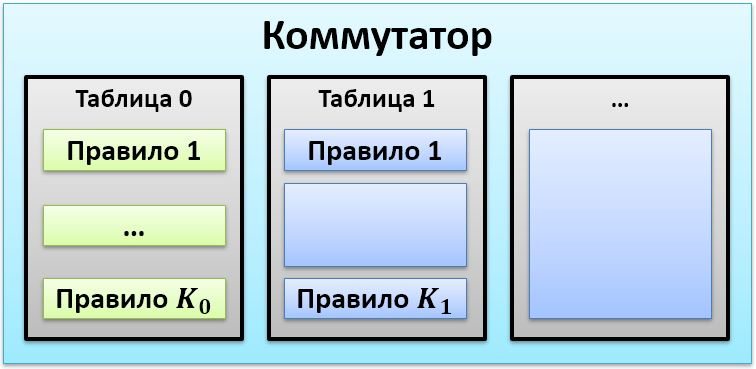
\includegraphics[width=0.6\textwidth]{figures/additionalrules.jpg}
\caption{Дополнительные правила маршрутизации} \label{fig:additionalrules}
\end{figure}

При отправке контроллеру ответов от коммутаторов, в ответах восстанавливается нулевая таблица для того, чтобы не нарушить работу приложений контроллера.

\pagebreak

\section{Анализ сетевой статистики}

Вторая фаза алгоритма обнаружения скомпрометированных коммутаторов предполагает предсказание значений счетчиков правил маршрутизации и сравнение этих значений с реальными, предоставляемыми коммутаторами в сети.

\subsection{Предсказание значений счетчиков}

Для предсказания значения счетчика правила, соответствующего некоторой вершине $v$ графа зависимостей правил, выполняется следующий набор действий:
\begin{enumerate}
\item Определяется набор $\mathcal{V}$ вершин путевой развертки, соответствующих вершине $v$ графа зависимостей правил;
\item Следуя по ветвям деревьев путевой развертки с корнями в множестве $\mathcal{V}$, выбираются вершины, соответствующие дополнительным правилам;
\item В сеть отправляются запросы статистики для набора выбранных дополнительных правил маршрутизации;
\item После получения статистики по дополнительным правилам маршрутизации выполняется алгоритм предсказания значений счетчиков (алгоритм \ref{alg:flow_propagation});
\item В качестве предсказанного значения счетчика правила, соответствующего вершине $v$, возвращается сумма значений потоков вершин из множества $\mathcal{V}$;
\item Значения потока в вершинах путевой развертки сохраняются для того, чтобы при новом запросе учитывать только изменение счетчика правила маршрутизации по сравнению с предыдущим значением.
\end{enumerate}

Необходимо отметить, что отличие в значениях счетчиков может появиться из-за легитимных потерь пакетов на портах коммутаторов.
Следовательно, нужно проверять, что пакеты были потеряны вследствие перегрузки, а не из-за компрометации коммутатора.

Все пакеты, потерянные из-за перегрузки, учитываются в счетчиках на портах коммутаторов.
Для проверки легитимности потерь трафика необходимо сравнить значение нехватки пакетов, полученное при предсказании счетчиков, и количество пакетов, потерянных на портах.
При сравнении необходимо учитывать только те порты, через которые проходят доменные пути, соответствующие проверяемому в данный момент правилу маршрутизации.

\subsection{Обнаружение скомпрометированных коммутаторов}

Для обнаружения скомпрометированного коммутатора из сети запрашивается реальное значение счетчика правила машрутизации и сравнивается с предсказанным значением.
Основная идея заключается в том, что при наличии в сети атаки на контур передачи данных эти значения будут отличаться.

\subsubsection{Сравнение значений счетчиков}

Каждому коммутатору присвоено значение $T\in [0,1]$, называемое \textit{уровнем доверия}.
Если уровень доверия некоторого коммутатора понижается ниже заданного порога, то регистрируется наличие в сети скомпрометированного коммутатора.

При несоответствии значений счетчиков уровни доверия изменяются следующим образом:
\begin{enumerate}
\item Выбираются коммутаторы, которые влияют на значение анализируемого счетчика правила маршрутизации;
    \begin{itemize}
    \item Для нахождения таких коммутаторов, алгоритм проходится по всем доменным путям, содержащим вершину, соответствующую анализируемому правилу.
    Вершины на этих путях влияют на значение анализируемого счетчика по теореме \ref{th:flow_decomposition}.
    \end{itemize}
\item Уровни доверия выбранных коммутаторов понижаются в $\delta$ раз.
\end{enumerate}

Если проверка правила прошла успешно, а именно, значения предсказанного и реального значения счетчика равны с учетом легитимных потерь пакетов, то уровни доверия коммутаторов, влияющих на этот счетчик, увеличиваются.
В данном случае увеличение уровня доверия будет аддитивное, то есть уровень увеличится на константу $\varepsilon$.

Таким образом, при успешной проверке уровни доверия будут увеличиваться аддитивно на константу $\varepsilon$, в то время как при неуспешной проверке, они будут уменьшаться мультипликативно в $\delta$ раз.

\subsubsection{Выбор правила для анализа}

В реальной сети может быть установлено большое количество правил маршрутизации, и проверка всех правил маршрутизации при каждом изменении состояния сети может создать дополнительную нагрузку на сеть.
Нагрузка на сеть появляется из-за того, что каждое предсказание значения счетчика требует набора запросов сетевой статистики к дополнительным правилам маршрутизации.

Для минимизации нагрузки на сеть используется рандомизированный механизм проверки правил.
Механизм заключается в следующем.
\begin{itemize}
\item Выбор правила для проверки значений счетчиков происходит случайно после фиксированного интервала времени;
\item Правило выбирается в зависимости от уровня доверия коммутатора, на котором оно установлено.
\end{itemize}

Вероятность $P_i$ выбора правила $r_i$ для проверки равна:
\begin{equation} \label{eq:checking_probability}
P_i = \frac{1 / T(v_i)}{\sum_{j\in [1,n]}{1 / T(v_j)}},
\end{equation}
где $T(v_i)$ --- уровень доверия коммутатора, на котором установлено правило $v_i$, а $n$ --- количество правил маршрутизации, установленных в сети.

Из \eqref{eq:checking_probability} следует, что при уменьшении уровней доверия некоторого коммутатора увеличивается вероятность проверки правила маршрутизации, установленного на этом коммутаторе, увеличивается.

\end{document}